% Generated from the report cells in Checkpoint1_notebook.ipynb.
% Edit this file directly for formatting, or regenerate with build_report.py.
% Compile from this directory: pdflatex Checkpoint1_report.tex
\documentclass[10pt,letterpaper]{article}
\usepackage[T1]{fontenc}
\usepackage{lmodern}
\usepackage[margin=0.8in,headheight=14pt,headsep=16pt,footskip=25pt]{geometry}
\usepackage{graphicx}
\usepackage{booktabs,tabularx,array}
\usepackage{enumitem}
\usepackage{float}
\usepackage{titlesec}
\usepackage[hidelinks]{hyperref}
\hypersetup{pdftitle={Checkpoint 1: First Results and Plan Revision},pdfauthor={CS 5593 Project Team}}
\urlstyle{same}
\setlength{\parindent}{0pt}
\setlength{\parskip}{4.5pt}
\setlength{\emergencystretch}{2em}
\linespread{1.04}
\titleformat{\section}{\large\bfseries}{\thesection.}{0.55em}{}
\titleformat{\subsection}[block]{\normalsize\bfseries}{}{0pt}{}
\titlespacing*{\section}{0pt}{14pt plus 2pt minus 1pt}{6pt}
\titlespacing*{\subsection}{0pt}{8pt}{5pt}
\setlist[enumerate]{leftmargin=1.5em,itemsep=5pt,topsep=4pt,parsep=0pt}
\pagestyle{plain}
\widowpenalty=10000
\clubpenalty=10000
\begin{document}
\begin{center}
{\LARGE\bfseries Checkpoint 1}\par
\vspace{4pt}
{\large First Results and Plan Revision}\par
\vspace{4pt}
{\normalsize Pickup and Sedan Listing Prices}\par
\vspace{3pt}
{\small CS 5593: Data Mining | Team Project}
\end{center}
\vspace{3pt}


\textbf{Research question:} Among U.S. Craigslist listings in April-May 2021, is the adjusted dollar decline in listing price per additional 10,000 miles smaller for pickups than for sedans, accounting for vehicle age, manufacturer, condition, transmission, and drivetrain?


\section{Progress Against Proposal}

Our proposal committed us to loading and cleaning the pickup/sedan listings, documenting missing and implausible values, creating vehicle-age and 10,000-mile mileage measures, and producing a cleaned dataset and exploratory summaries. We completed these steps for 119,016 listings (40,481 pickups and 78,535 sedans) and exported the cleaned dataset. A fresh download from the proposal's Kaggle source reproduces the original dimensions and group counts; we retain the original question and document the cleaning and missing-data assumptions that need further checks.


\section{Method Implemented}

\subsection*{Data and workflow}

We use the \texttt{vehicles.csv} file from Austin Reese's \href{https://www.kaggle.com/datasets/austinreese/craigslist-carstrucks-data}{Used Cars Dataset on Kaggle}, the source linked in our proposal. The source has 426,880 listings and 26 columns; we load the 12 columns needed for analysis, date checks, and listing/vehicle identification. We retain the exact \texttt{pickup} and \texttt{sedan} categories, giving 130,566 listings before numeric cleaning; the separate \texttt{truck} category is outside our stated subset. Non-missing posting dates fall in April-May 2021, and none of the pickup/sedan listings lacks a posting date.


Each observation is one listing, not necessarily one unique vehicle. We check listing URLs and IDs for duplication and separately count repeated non-missing VINs. We retain distinct listings, but repeated vehicles can give some vehicles extra weight and will require a sensitivity check before statistical inference.


\begin{minipage}{\linewidth}
\subsection*{Preprocessing and representation}
\begin{center}
\small
\renewcommand{\arraystretch}{1.18}
\begin{tabularx}{\linewidth}{@{}>{\raggedright\arraybackslash}p{0.19\linewidth}>{\raggedright\arraybackslash}p{0.34\linewidth}>{\raggedright\arraybackslash}X@{}}
\toprule
\textbf{Step} & \textbf{Input and rule} & \textbf{Output and reason} \\
\midrule
Date and type selection & Raw listings; keep observed dates and exact pickup/sedan labels & Listings in the proposed period and categories \\
Required numeric fields & Exclude missing price, odometer, or model year & Records with observed outcome, mileage, and age inputs \\
Price restriction & Keep \$101-\$100,000, inclusive & Remove very low placeholder-like prices and extreme prices; some genuine listings may be excluded \\
Mileage restriction & Keep 1-400,000 miles, inclusive & Remove nonpositive readings and extreme mileage while retaining plausible high-mileage vehicles \\
Model-year restriction & Keep 1900-2021, inclusive & Define nonnegative model-year age relative to 2021; 2022 models can exist in 2021 but are outside this age definition \\
Missing categories & Replace missing manufacturer, condition, transmission, and drive with \texttt{unknown} & Preserve listings and record missing information explicitly \\
Derived features & Age = 2021 minus model year; mileage = odometer divided by 10,000 & Comparable age and mileage units for the planned model \\
\bottomrule
\end{tabularx}
\end{center}
\end{minipage}

The 300,000-mile diagnostic is a flag for inspection, not the exclusion threshold. The final ceiling is 400,000 miles to preserve high-mileage listings relevant to the question; its influence remains to be checked. Pre-1990 vehicles are retained rather than assumed erroneous, but their price relationship may differ from ordinary used vehicles. These are preliminary analytic restrictions, not proof that every retained value is valid or every excluded value is an error. The sequential audit below applies the same final rules and counts each excluded listing once.


The resulting table has 119,016 listings and 11 columns, including the ID. Labeling missing categories \texttt{unknown} does not recover their values; we retain this category for later encoding rather than interpolating nominal labels.


\subsection*{Analysis completed and connection to the question}

We calculate counts, missing-value totals, quantiles, and group summaries, then compare listing price, mileage, and age between pickups and sedans. The cleaned listing table is the input; the outputs are a cleaning audit, group comparison table, and exploratory mileage-price figure. These summaries check whether the proposed comparison is feasible and expose distribution differences; they do not estimate the adjusted mileage effect. The multiple linear regression and mileage-by-type interaction remain the next checkpoint's analysis.


\begin{minipage}{\linewidth}
\subsection*{Sequential cleaning audit}
\begin{center}
\small
\renewcommand{\arraystretch}{1.18}
\begin{tabularx}{\linewidth}{@{}>{\raggedright\arraybackslash}X>{\raggedleft\arraybackslash}p{0.20\linewidth}>{\raggedleft\arraybackslash}p{0.20\linewidth}@{}}
\toprule
\textbf{Exclusion step, in order} & \textbf{Removed at this step} & \textbf{Remaining} \\
\midrule
Missing required numeric values & 2,120 & 128,446 \\
Price outside \$101-\$100,000 & 8,987 & 119,459 \\
Odometer outside 1-400,000 miles & 443 & 119,016 \\
Model year outside 1900-2021 & 0 & 119,016 \\
\bottomrule
\end{tabularx}
\end{center}
\end{minipage}

Starting subset: 130,566 listings. Total removed: 11,550. Counts depend on the displayed order and do not overlap; a zero in the final row means no additional records fail that rule after earlier exclusions.


\section{Preliminary Results}

\begin{minipage}{\linewidth}
\subsection*{Group comparison}
\begin{center}
\small
\renewcommand{\arraystretch}{1.18}
\begin{tabularx}{\linewidth}{@{}>{\raggedright\arraybackslash}X>{\raggedleft\arraybackslash}p{0.20\linewidth}>{\raggedleft\arraybackslash}p{0.20\linewidth}@{}}
\toprule
\textbf{Measure} & \textbf{Pickups} & \textbf{Sedans} \\
\midrule
Before numeric cleaning & 43,510 & 87,056 \\
After numeric cleaning & 40,481 & 78,535 \\
Excluded by numeric cleaning & 3,029 (6.96\%) & 8,521 (9.79\%) \\
Median listing price & \$27,995 & \$10,999 \\
Mean mileage & 85,517 miles & 86,098 miles \\
Median mileage & 70,559 miles & 81,675 miles \\
Median model-year age & 6 years & 7 years \\
\bottomrule
\end{tabularx}
\end{center}
\end{minipage}

The group comparison is computed from the verified Kaggle source. Numeric cleaning retains 119,016 of 130,566 pickup/sedan listings, removing 11,550 (8.85\%). The sequential audit records each exclusion once rather than summing overlapping diagnostic flags.


Pickups have a much higher median listing price. Mean mileage is similar between the groups, but the median pickup has 11,116 fewer miles and is one model year younger. These differences make separate group summaries useful and motivate accounting for age and other characteristics before comparing mileage slopes. Higher pickup prices alone do not show that their prices decline less per 10,000 miles.


\subsection*{Exploratory price-mileage comparison}

Figure 1 displays price against mileage in units of 10,000 miles, with the same axes for both groups. A reproducible sample of 3,500 listings per group keeps the points readable; the overlaid medians use all retained listings in 20,000-mile bins with at least 30 observations. These are unadjusted descriptive summaries, not fitted regression effects.


\begin{figure}[H]
\centering
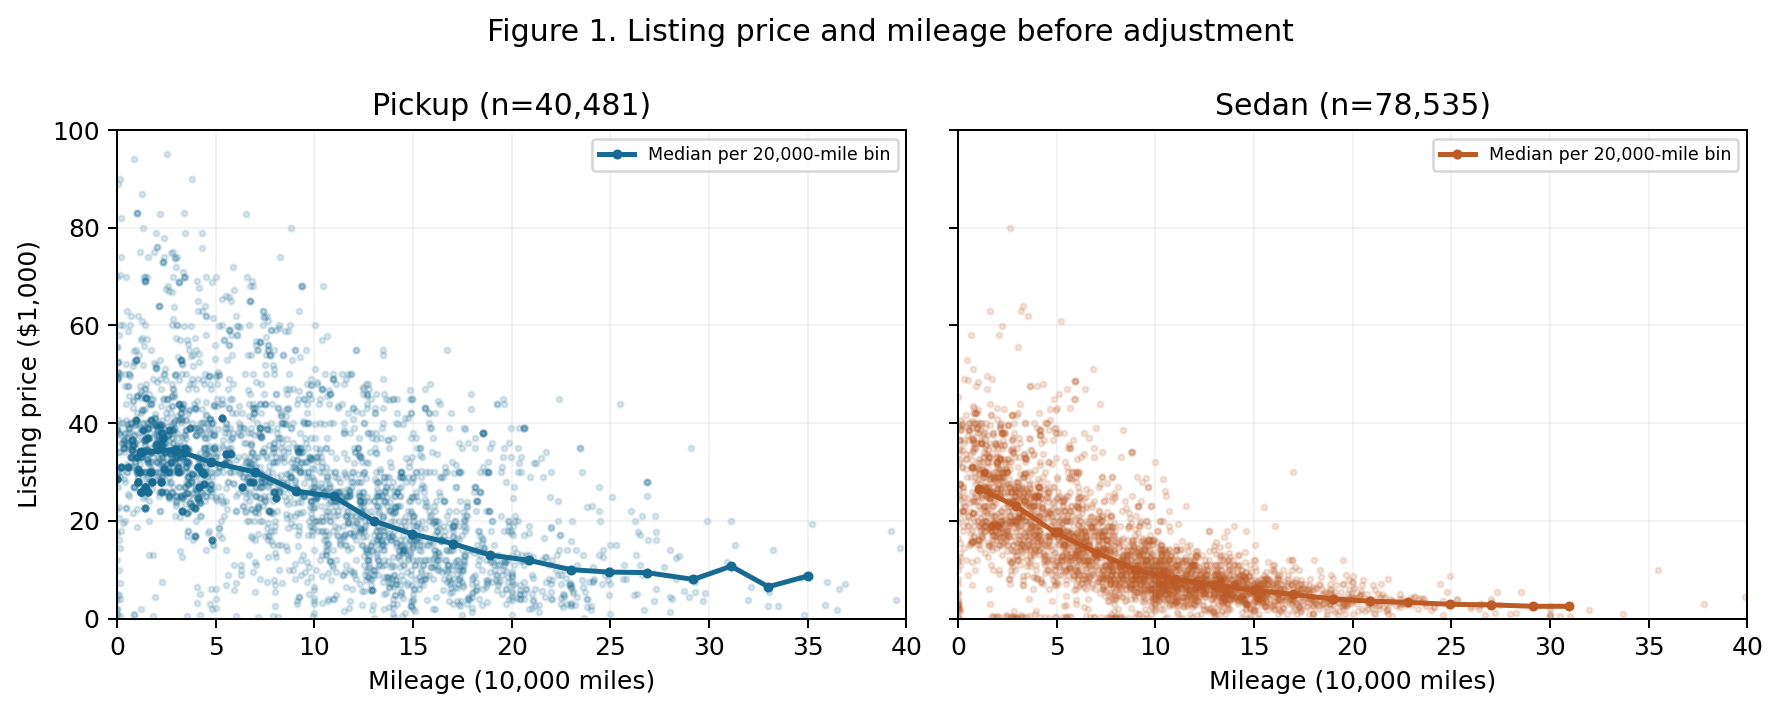
\includegraphics[width=\linewidth]{figures/price_mileage.png}
\end{figure}

Across most mileage bins, median listing prices decrease for both vehicle types, while pickups remain more expensive. The curves flatten at higher mileage and the pickup tail is uneven, so a single constant dollar decline may be an approximation. These exploratory relationships motivate the proposed adjusted comparison, but neither the raw curves nor the price gap establishes that pickups have a smaller adjusted decline per 10,000 miles.


\subsection*{Limitations and uncertainty}

Before numeric cleaning, condition is missing for 44,092 listings (33.77\%) and drive for 28,275 (21.66\%). An \texttt{unknown} category preserves listings but cannot fully account for the missing characteristics. The retained data also include 1,786 prices at or below \$500, 606 mileage readings at or below 100 miles, and vehicles up to 98 model years old. These may include unusual genuine listings and reporting errors, so our numeric bounds do not guarantee a homogeneous used-vehicle sample.


Cleaning excludes 9.79\% of sedans versus 6.96\% of pickups. This difference does not establish bias, but it requires checking whether the comparison depends on filtering choices. Repeated vehicles across distinct listings may also affect weighting and uncertainty. Our evidence concerns asking prices on Craigslist in the specified period, not completed sale prices or the same vehicle losing value over time.


\textbf{Course connection:} The group table uses the descriptive statistics and quantiles in the Week 1 reading (pp. 15-23); the figure follows its scatterplot discussion (p. 29). We interpret unusual values as observations to investigate rather than automatically treating every extreme as an error, following Week 1\_3 (p. 7).


\section{Evaluation of the Original Hypothesis and Plan}

Our hypothesis remains unresolved: we have not yet estimated the adjusted difference in dollar decline per 10,000 miles. The broad downward price-mileage patterns are consistent with the expectation that higher-mileage listings tend to have lower prices, but they do not establish the predicted smaller decline for pickups. The higher pickup price level is a different quantity from the mileage slope.


The proposal's first steps remain useful. Both groups retain large samples, the required numeric measures can be constructed, and the observed price, mileage, and age differences justify retaining the proposed adjustment for vehicle characteristics. We therefore preserve the original research question and use the mileage-by-type regression as the next comparison.


The data challenge several simplifying assumptions. Missing condition and drive information limits adjustment; suspicious retained prices and odometer readings require inspection; and differential exclusions and repeated vehicles may affect the comparison. We also need to define how listings marked new and very old vehicles fit the used-vehicle population. The curved binned patterns suggest checking whether a single linear mileage slope and linear age adjustment adequately describe the data rather than assuming they do.


These findings call for refining validation and interpretation, not declaring the hypothesis confirmed or rejected. Following Week 1\_3 (pp. 3-8), we distinguish the Craigslist sample from the broader vehicle market, consider selection and confounding, and treat the observed patterns as associations rather than causal depreciation.


\section{Next-Step Plan or Revision}

We will continue the original research question and planned interaction regression, while refining the data checks and verifying that the model represents the observed relationships.


\begin{enumerate}

\item \textbf{Review questionable listings and define the analytic population.} Inspect low-price and near-zero-mileage records, listings marked new, and very old vehicles. Document which are usable for the stated used-vehicle question. Compare the primary analysis with reasonable alternative restrictions and with repeated known-VIN listings reduced to one listing per vehicle, reporting the remaining limitation for missing VINs. This follows from the retained anomalies and unequal cleaning losses.

\item \textbf{Prepare the proposed adjusted comparison.} Encode manufacturer, condition, transmission, and drive as categorical indicators, retaining \texttt{unknown} explicitly. Fit listing price in dollars using mileage in 10,000-mile units, pickup/sedan type, their interaction, vehicle age, and the four categorical controls. Use sedan as the reference group. The mileage coefficient estimates the sedan slope; adding the interaction gives the pickup slope. A positive interaction supports a smaller pickup decline only when the estimated slopes describe declines and the uncertainty supports the difference.

\item \textbf{Check interpretation and model adequacy.} Examine residual patterns and whether age and mileage need more flexible representations, because the exploratory curves are not straight. Compare conclusions across the documented data restrictions and report both slopes, their difference, and confidence intervals using uncertainty estimates that account for unequal residual variation and repeated vehicles where identifiable. Do not treat statistical significance alone as practical importance.

\end{enumerate}

The next artifacts will be a documented sensitivity comparison, the two adjusted dollar changes per 10,000 miles and their difference with uncertainty, and a grouped mileage-price visualization with clearly labeled adjusted predictions. These outputs directly address the proposed hypothesis while preserving the distinction between listing-price association and causal depreciation.


\subsection*{Sources and verification}

\textbf{Dataset:} Austin Reese, Used Cars Dataset, Kaggle: \newline\url{https://www.kaggle.com/datasets/austinreese/craigslist-carstrucks-data}. Downloaded October 16, 2026; file checksum and download details are recorded in \texttt{data/source.json}.


\textbf{Project requirements:} Team Research Proposal, Checkpoint 1 commitment; CS 5593 Team Project: Checkpoint 1, First Results and Plan Revision, pp. 1-2.


\textbf{Course material:} Week 1 reading, pp. 15-23 and 29 (descriptive statistics, quantiles, and scatterplots); Week 1\_3, pp. 3-8 (sample selection, association, confounding, unusual observations, and analytical validity).


\textbf{Verification:} The downloaded source reproduces 426,880 rows, 26 columns, April-May posting counts, 130,566 pickup/sedan listings before numeric cleaning, and 119,016 after cleaning. All 26 code cells executed successfully; the exported group summary, cleaning audit, and figure come from that execution. No adjusted regression result is claimed at this checkpoint.


\end{document}
